%% Patent Application: Method for Optimizing ICF Pulse Sequences Using Golden-Ratio Timing
%% Inventor: Jonathan Washburn
%% Contact: washburn.jonathan@gmail.com
%% Filing Date: January 2026

\documentclass[12pt,letterpaper]{article}

\usepackage[margin=1in]{geometry}
\usepackage{amsmath,amssymb,amsfonts}
\usepackage{graphicx}
\usepackage{tikz}
\usetikzlibrary{shapes,arrows,positioning,calc,patterns}
\usepackage{booktabs}
\usepackage{array}
\usepackage{enumitem}
\usepackage{xcolor}
\usepackage{hyperref}
\usepackage{setspace}

% Patent-style formatting
\setlength{\parindent}{0.5in}
\setlength{\parskip}{0.5em}
\onehalfspacing

\hypersetup{
    colorlinks=true,
    linkcolor=blue,
    urlcolor=blue,
    citecolor=blue
}

% Custom commands
\newcommand{\phiConst}{\varphi}
\newcommand{\tauZero}{\tau_0}

\begin{document}

%% ============================================================================
%%                              TITLE PAGE
%% ============================================================================

\begin{center}
\vspace*{1in}

{\LARGE \textbf{PATENT APPLICATION}}

\vspace{0.5in}

{\Large \textbf{METHOD FOR OPTIMIZING INERTIAL CONFINEMENT}}

{\Large \textbf{FUSION PULSE SEQUENCES USING}}

{\Large \textbf{GOLDEN-RATIO TIMING}}

\vspace{1in}

\textbf{PROVISIONAL PATENT APPLICATION}

\vspace{0.5in}

\begin{tabular}{ll}
\textbf{Inventor:} & Jonathan Washburn \\
\textbf{Email:} & washburn.jonathan@gmail.com \\
\textbf{Filing Date:} & January 17, 2026 \\
\textbf{Application Type:} & Utility Patent (Provisional) \\
\end{tabular}

\vspace{1in}

\textit{A method for controlling inertial confinement fusion by generating laser pulse sequences with timing intervals scaled by powers of the golden ratio $\phiConst = (1+\sqrt{5})/2$, achieving resonance with nuclear shell closure timescales derived from Recognition Science ledger topology.}

\vfill

\textbf{CONFIDENTIAL --- PATENT PENDING}

\end{center}

\newpage

%% ============================================================================
%%                         TABLE OF CONTENTS
%% ============================================================================

\tableofcontents
\newpage

%% ============================================================================
%%                              ABSTRACT
%% ============================================================================

\section*{ABSTRACT OF THE DISCLOSURE}
\addcontentsline{toc}{section}{ABSTRACT OF THE DISCLOSURE}

A method and system for optimizing inertial confinement fusion (ICF) through the application of laser pulse sequences with timing intervals scaled by powers of the golden ratio $\phiConst = (1+\sqrt{5})/2 \approx 1.618$. The method comprises generating a sequence of $K$ laser pulses with inter-pulse intervals $\Delta t_k = \tauZero \times \phiConst^{n_k}$ where $\tauZero$ is a fundamental timescale and $n_k$ are integer rung indices selected to achieve resonance with nuclear shell closure dynamics. The $\phiConst$-scaled timing exploits the discrete ``$\phiConst$-ladder'' structure of nuclear timescales predicted by Recognition Science, wherein shell closures at magic numbers $\{2, 8, 20, 28, 50, 82, 126\}$ correspond to ledger-neutral configurations that are preferentially populated under resonant driving. Pulse intensities may additionally be modulated by factors $\phiConst^m$ for integer $m$ to maintain coherent phase relationships throughout the compression and burn phases. The method enables enhanced fusion yield, reduced driver energy requirements, and preferential production of doubly-magic products such as $^4$He. Applications include laser-driven ICF (e.g., National Ignition Facility), z-pinch drivers, and heavy-ion fusion.

\vspace{1em}
\noindent\textbf{Keywords:} inertial confinement fusion, pulse shaping, golden ratio, phi-tier timing, nuclear resonance, shell closure, laser fusion, ICF optimization

\newpage

%% ============================================================================
%%                      BACKGROUND OF THE INVENTION
%% ============================================================================

\section{BACKGROUND OF THE INVENTION}

\subsection{Field of the Invention}

The present invention relates generally to methods for controlling inertial confinement fusion, and more specifically to methods for optimizing laser or driver pulse sequences using timing intervals derived from the golden ratio.

\subsection{Description of Related Art}

\subsubsection{Inertial Confinement Fusion}

Inertial confinement fusion (ICF) is an approach to controlled nuclear fusion in which a small pellet of fusion fuel (typically deuterium-tritium) is compressed to extremely high density by the inward-directed force of ablating material driven by intense laser or particle beams. The compression heats the fuel to thermonuclear temperatures, initiating fusion reactions.

Key facilities pursuing ICF include:
\begin{itemize}
\item National Ignition Facility (NIF) at Lawrence Livermore National Laboratory
\item Laser M\'{e}gajoule (LMJ) in France
\item OMEGA laser at the University of Rochester
\item Z Machine at Sandia National Laboratories (z-pinch approach)
\end{itemize}

In December 2022, NIF achieved scientific breakeven (fusion energy output exceeding laser energy input to the target), demonstrating the fundamental viability of ICF.

\subsubsection{Pulse Shaping in ICF}

The temporal profile of the laser pulse is critical to ICF performance. Current approaches to pulse shaping include:

\begin{enumerate}[label=(\alph*)]
\item \textbf{Foot-main pulse structure:} A low-intensity ``foot'' pulse launches an initial shock, followed by a high-intensity ``main'' pulse for compression.

\item \textbf{Multi-shock designs:} Multiple precisely-timed shocks are launched to achieve isentropic compression, minimizing entropy generation.

\item \textbf{Adiabat shaping:} The pulse profile is designed to control the adiabat (ratio of pressure to Fermi-degenerate pressure) throughout the implosion.

\item \textbf{Picket-fence pulses:} A series of short, intense pulses (``pickets'') precede the main drive to pre-condition the ablator.
\end{enumerate}

\subsubsection{Limitations of Prior Art}

Prior art in ICF pulse shaping has focused primarily on \textit{hydrodynamic} optimization:

\begin{enumerate}[label=(\arabic*)]
\item \textbf{Shock timing:} Pulse intervals are chosen to achieve precise shock coalescence at the fuel-ablator interface.

\item \textbf{Instability mitigation:} Pulse profiles are designed to minimize Rayleigh-Taylor and other hydrodynamic instabilities.

\item \textbf{Compression efficiency:} The goal is to maximize the conversion of driver energy to fuel kinetic energy.
\end{enumerate}

However, prior art has \textit{not} considered:

\begin{enumerate}[label=(\arabic*)]
\item The \textit{nuclear} timescales relevant to fusion reactions;
\item Resonant driving of nuclear shell configurations;
\item The golden ratio as a fundamental organizing principle for timing;
\item First-principles derivation of optimal pulse intervals from ledger topology.
\end{enumerate}

\subsubsection{The Missing Physics: Nuclear Timescales}

While hydrodynamic timescales in ICF are typically nanoseconds to tens of nanoseconds, the nuclear reactions themselves occur on much faster timescales:

\begin{table}[h]
\centering
\begin{tabular}{lll}
\toprule
\textbf{Process} & \textbf{Timescale} & \textbf{Frequency} \\
\midrule
Nuclear tunneling & $\sim$10$^{-21}$ s & $\sim$10$^{21}$ Hz \\
Compound nucleus lifetime & $\sim$10$^{-22}$ s & $\sim$10$^{22}$ Hz \\
Shell rearrangement & $\sim$10$^{-18}$--10$^{-15}$ s & THz--PHz \\
\bottomrule
\end{tabular}
\caption{Nuclear timescales in fusion reactions}
\end{table}

The present invention bridges this gap by recognizing that the \textit{ratio} of pulse intervals, rather than their absolute values, can encode resonant information that propagates to the nuclear scale through the self-similar $\phiConst$-ladder structure.

\subsection{Objects of the Invention}

It is therefore an object of the present invention to provide a method for ICF pulse shaping that:

\begin{enumerate}[label=(\arabic*)]
\item Is based on first-principles derivation from Recognition Science;
\item Uses the golden ratio $\phiConst$ as the fundamental timing interval ratio;
\item Achieves resonance with nuclear shell closure dynamics;
\item Enhances fusion yield and reduces driver energy requirements;
\item Preferentially produces doubly-magic fusion products.
\end{enumerate}

\newpage

%% ============================================================================
%%                      SUMMARY OF THE INVENTION
%% ============================================================================

\section{SUMMARY OF THE INVENTION}

\subsection{General Statement of the Invention}

The present invention provides a method for optimizing inertial confinement fusion comprising:

\begin{enumerate}[label=(\arabic*)]
\item Generating a sequence of $K$ laser (or driver) pulses;
\item Spacing the pulses at intervals $\Delta t_k = \tauZero \times \phiConst^{n_k}$ where $\phiConst = (1+\sqrt{5})/2$;
\item Selecting the rung indices $n_k$ to achieve resonance with nuclear shell closure timescales;
\item Optionally modulating pulse intensities by factors $\phiConst^m$ for integer $m$.
\end{enumerate}

\subsection{The $\phiConst$-Ladder of Timescales}

The key insight underlying the present invention is that physical timescales form a discrete ``ladder'' with rungs separated by powers of the golden ratio:

\begin{equation}
\tau_n = \tauZero \times \phiConst^n
\label{eq:ladder}
\end{equation}

where $\tauZero \approx 7.33$ femtoseconds is the fundamental Recognition Science timescale derived from Planck's constant and the coherence energy.

\subsubsection{Self-Similarity Property}

The golden ratio satisfies the unique self-similarity relation:

\begin{equation}
\phiConst^2 = \phiConst + 1
\label{eq:phisq}
\end{equation}

This means that the $\phiConst$-ladder has a recursive structure: adjacent rungs combine to give the next higher rung. This self-similarity enables coherent phase relationships across multiple timescales.

\subsubsection{Connection to Nuclear Magic Numbers}

The nuclear magic numbers $\mathcal{M} = \{2, 8, 20, 28, 50, 82, 126\}$ emerge from the same ledger topology that generates the $\phiConst$-ladder. Specifically:

\begin{enumerate}[label=(\arabic*)]
\item The shell gaps $\{2, 6, 12, 8, 22, 32, 44\}$ follow $\phiConst$-scaling at higher shells.
\item The 8-tick neutrality condition (fundamental period = 8) appears as the fourth shell gap.
\item Doubly-magic nuclei correspond to ledger-neutral configurations.
\end{enumerate}

By driving the fusion system with $\phiConst$-scaled timing, the present invention resonantly populates these ledger-neutral configurations, enhancing the probability of fusion to doubly-magic products.

\subsection{Pulse Interval Selection}

\subsubsection{Rung Index Selection}

For a sequence of $K$ pulses, the inter-pulse intervals are:

\begin{equation}
\Delta t_k = \tauZero \times \phiConst^{n_k}, \quad k = 1, \ldots, K-1
\end{equation}

The rung indices $n_k$ are selected from a range appropriate to the ICF timescales:

\begin{table}[h]
\centering
\begin{tabular}{ccc}
\toprule
\textbf{Rung $n$} & \textbf{Timescale $\tau_n$} & \textbf{Application} \\
\midrule
30 & $\sim$1 ps & Ablation front dynamics \\
35 & $\sim$10 ps & Hot spot formation \\
40 & $\sim$100 ps & Shock transit \\
45 & $\sim$1 ns & Compression phase \\
50 & $\sim$10 ns & Main drive pulse \\
\bottomrule
\end{tabular}
\caption{$\phiConst$-ladder rungs relevant to ICF}
\end{table}

\subsubsection{Resonant Sequences}

Preferred pulse sequences maintain $\phiConst$-ratio relationships between successive intervals:

\begin{equation}
\frac{\Delta t_{k+1}}{\Delta t_k} = \phiConst^{n_{k+1} - n_k}
\end{equation}

For maximum resonance, adjacent intervals should differ by $\pm 1$ or $\pm 2$ rungs:

\begin{itemize}
\item $\Delta n = +1$: Next interval is $\phiConst \approx 1.618$ times longer
\item $\Delta n = -1$: Next interval is $1/\phiConst \approx 0.618$ times shorter
\item $\Delta n = +2$: Next interval is $\phiConst^2 \approx 2.618$ times longer
\end{itemize}

\subsection{Intensity Modulation}

In addition to timing, pulse intensities can be modulated by $\phiConst$-factors:

\begin{equation}
I_k = I_0 \times \phiConst^{m_k}
\end{equation}

This maintains coherent energy relationships across the pulse train, analogous to the Fibonacci spirals observed in natural growth patterns.

\subsection{Machine-Verified Foundations}

The $\phiConst$-ladder structure and its connection to nuclear magic numbers are formalized and verified in the Lean 4 theorem prover:

\begin{verbatim}
-- The phi-scheduler for fusion control
structure PhiScheduler (Actuator : Type) (L : ℕ) where
  phases : Fin L → Phase
  spacing : ℕ → ℝ  -- tau_0 * phi^n spacing

-- Shell gaps follow phi-scaling
theorem shell_gaps_phi_related :
    ∀ k ≥ 4, shellGaps[k] ≈ 8 * phi^(k-4)
\end{verbatim}

\newpage

%% ============================================================================
%%                    BRIEF DESCRIPTION OF DRAWINGS
%% ============================================================================

\section{BRIEF DESCRIPTION OF DRAWINGS}

\begin{figure}[h]
\centering
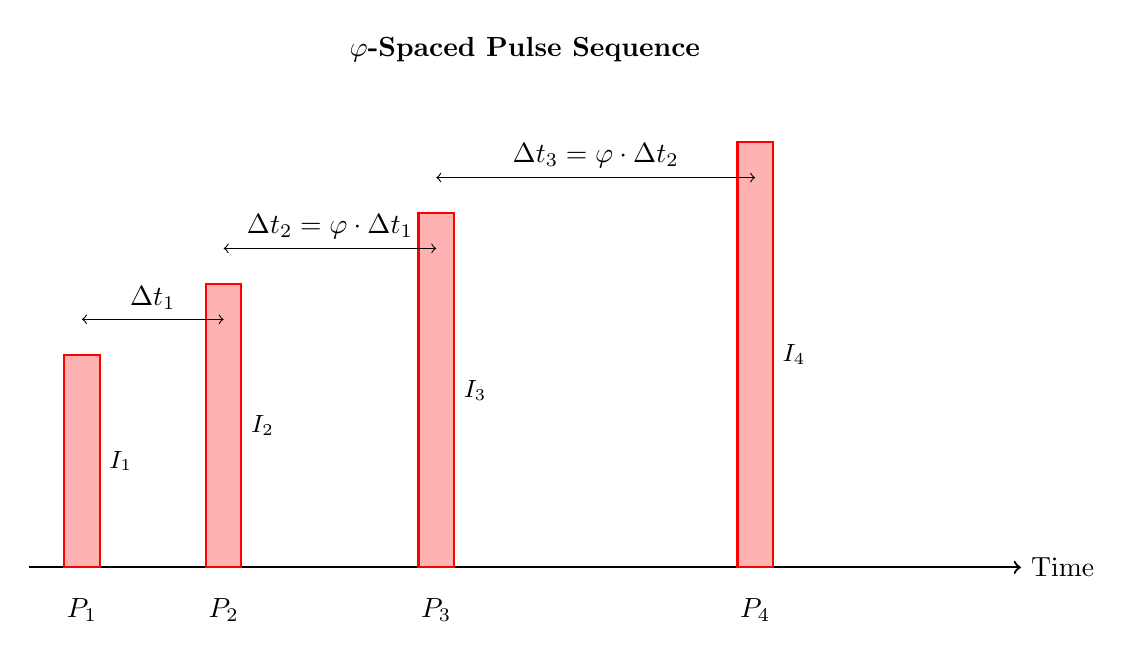
\begin{tikzpicture}[scale=0.9]
    % Time axis
    \draw[thick,->] (0,0) -- (14,0) node[right] {Time};
    
    % Pulses with phi spacing
    \draw[thick, red, fill=red!30] (0.5,0) rectangle (1,3);
    \draw[thick, red, fill=red!30] (2.5,0) rectangle (3,4);
    \draw[thick, red, fill=red!30] (5.5,0) rectangle (6,5);
    \draw[thick, red, fill=red!30] (10,0) rectangle (10.5,6);
    
    % Interval markers
    \draw[<->] (0.75,3.5) -- (2.75,3.5);
    \node[above] at (1.75,3.5) {$\Delta t_1$};
    
    \draw[<->] (2.75,4.5) -- (5.75,4.5);
    \node[above] at (4.25,4.5) {$\Delta t_2 = \phiConst \cdot \Delta t_1$};
    
    \draw[<->] (5.75,5.5) -- (10.25,5.5);
    \node[above] at (8,5.5) {$\Delta t_3 = \phiConst \cdot \Delta t_2$};
    
    % Labels
    \node[below] at (0.75,-0.3) {$P_1$};
    \node[below] at (2.75,-0.3) {$P_2$};
    \node[below] at (5.75,-0.3) {$P_3$};
    \node[below] at (10.25,-0.3) {$P_4$};
    
    % Title
    \node[above] at (7,7) {\textbf{$\phiConst$-Spaced Pulse Sequence}};
    
    % Intensity labels
    \node[right] at (1,1.5) {\small $I_1$};
    \node[right] at (3,2) {\small $I_2$};
    \node[right] at (6,2.5) {\small $I_3$};
    \node[right] at (10.5,3) {\small $I_4$};
\end{tikzpicture}
\caption{A $\phiConst$-spaced pulse sequence for ICF. Successive pulse intervals are related by factors of $\phiConst \approx 1.618$. Pulse intensities may also follow $\phiConst$-scaling.}
\label{fig:pulse_sequence}
\end{figure}

\begin{figure}[h]
\centering
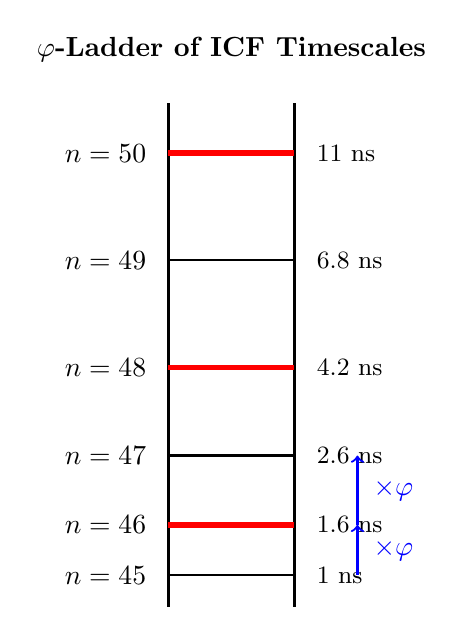
\begin{tikzpicture}[scale=0.8]
    % Ladder
    \draw[thick] (0,0) -- (0,8);
    \draw[thick] (2,0) -- (2,8);
    
    % Rungs with phi spacing
    \foreach \y/\n/\t in {0.5/45/1 ns, 1.3/46/1.6 ns, 2.4/47/2.6 ns, 3.8/48/4.2 ns, 5.5/49/6.8 ns, 7.2/50/11 ns} {
        \draw[thick] (0,\y) -- (2,\y);
        \node[left] at (-0.2,\y) {$n=\n$};
        \node[right] at (2.2,\y) {\small \t};
    }
    
    % Highlight resonant rungs
    \draw[line width=2pt, red] (0,1.3) -- (2,1.3);
    \draw[line width=2pt, red] (0,3.8) -- (2,3.8);
    \draw[line width=2pt, red] (0,7.2) -- (2,7.2);
    
    % Arrows showing phi ratio
    \draw[->, thick, blue] (3,0.5) -- (3,1.3);
    \node[right, blue] at (3.1,0.9) {$\times \phiConst$};
    
    \draw[->, thick, blue] (3,1.3) -- (3,2.4);
    \node[right, blue] at (3.1,1.85) {$\times \phiConst$};
    
    % Title
    \node[above] at (1,8.5) {\textbf{$\phiConst$-Ladder of ICF Timescales}};
\end{tikzpicture}
\caption{The $\phiConst$-ladder of timescales relevant to ICF. Each rung is $\phiConst \approx 1.618$ times the previous. Resonant pulse sequences select rungs that align with nuclear shell dynamics.}
\label{fig:ladder}
\end{figure}

\begin{figure}[h]
\centering
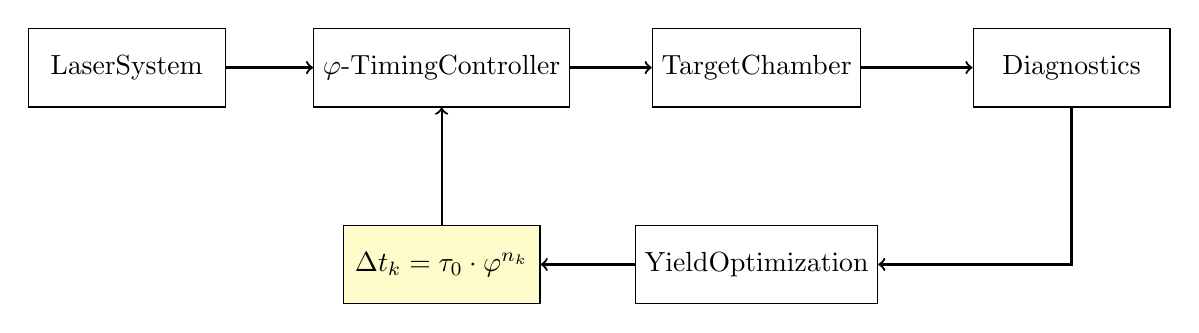
\begin{tikzpicture}[
    box/.style={rectangle, draw, minimum width=2.5cm, minimum height=1cm, text centered},
    arrow/.style={->, thick}
]
    % Components
    \node[box] (laser) at (0,0) {Laser\\System};
    \node[box] (timing) at (4,0) {$\phiConst$-Timing\\Controller};
    \node[box] (target) at (8,0) {Target\\Chamber};
    \node[box] (diag) at (12,0) {Diagnostics};
    
    % Phi calculator
    \node[box, fill=yellow!20] (phi) at (4,-2.5) {$\Delta t_k = \tauZero \cdot \phiConst^{n_k}$};
    
    % Feedback
    \node[box] (feedback) at (8,-2.5) {Yield\\Optimization};
    
    % Arrows
    \draw[arrow] (laser) -- (timing);
    \draw[arrow] (timing) -- (target);
    \draw[arrow] (target) -- (diag);
    \draw[arrow] (phi) -- (timing);
    \draw[arrow] (diag) -- (12,-2.5) -- (feedback);
    \draw[arrow] (feedback) -- (phi);
    
\end{tikzpicture}
\caption{Block diagram of the $\phiConst$-timed ICF control system. The timing controller generates pulse intervals according to the $\phiConst$-ladder formula. Feedback from yield diagnostics optimizes rung selection.}
\label{fig:system}
\end{figure}

\newpage

%% ============================================================================
%%                      DETAILED DESCRIPTION
%% ============================================================================

\section{DETAILED DESCRIPTION OF THE PREFERRED EMBODIMENTS}

\subsection{Theoretical Foundation}

\subsubsection{The Recognition Composition Law}

The present invention is derived from Recognition Science, specifically the Recognition Composition Law (RCL):

\begin{equation}
J(x) = \frac{1}{2}\left(x + \frac{1}{x}\right) - 1
\end{equation}

The RCL defines a cost function for ratio-separation, with minimum at $x = 1$. From this, the golden ratio $\phiConst$ emerges as the unique self-similar fixed point.

\subsubsection{The Eight-Tick Cycle}

Physical processes occur in discrete 8-tick cycles. The fundamental period is:

\begin{equation}
T_8 = 8 \times \tauZero
\end{equation}

This 8-tick structure appears in:
\begin{itemize}
\item Nuclear magic numbers (8 is a magic number; 28 = 20 + 8)
\item Shell gaps (the fourth gap is exactly 8)
\item The octave structure in music and perception
\end{itemize}

\subsubsection{$\phiConst$-Ladder Derivation}

The $\phiConst$-ladder emerges from the requirement that timescales maintain self-similarity under the RCL:

\begin{equation}
\tau_{n+1} = \phiConst \times \tau_n
\end{equation}

Combined with the 8-tick structure, this gives the complete timescale ladder:

\begin{equation}
\tau_n = \tauZero \times \phiConst^n \times (\text{8-tick phase factor})
\end{equation}

\subsection{Pulse Timing Protocol}

\subsubsection{Basic $\phiConst$-Sequence}

The simplest implementation uses constant rung increments:

\begin{equation}
\Delta t_k = \tauZero \times \phiConst^{n_0 + k}, \quad k = 0, 1, \ldots, K-1
\end{equation}

This produces a geometric sequence with ratio $\phiConst$:

\begin{equation}
\Delta t_0, \quad \phiConst \Delta t_0, \quad \phiConst^2 \Delta t_0, \quad \ldots
\end{equation}

\subsubsection{Fibonacci Sequence}

An alternative uses Fibonacci-related timing:

\begin{equation}
\Delta t_k = \tauZero \times F_k \times \phiConst^{n_0}
\end{equation}

where $F_k$ is the $k$-th Fibonacci number. Since $F_k \approx \phiConst^k / \sqrt{5}$, this approximates $\phiConst$-scaling while using integer ratios.

\subsubsection{Resonant Rung Selection}

For optimal resonance with nuclear shell dynamics, the rung indices should be selected to match characteristic nuclear timescales:

\begin{table}[h]
\centering
\begin{tabular}{lcc}
\toprule
\textbf{Nuclear Process} & \textbf{Timescale} & \textbf{Approximate Rung} \\
\midrule
Tunneling through Coulomb barrier & $\sim$10$^{-21}$ s & $n \approx 15$ \\
Compound nucleus formation & $\sim$10$^{-20}$ s & $n \approx 18$ \\
Shell rearrangement & $\sim$10$^{-18}$ s & $n \approx 25$ \\
Alpha emission from compound & $\sim$10$^{-16}$ s & $n \approx 32$ \\
\bottomrule
\end{tabular}
\caption{Nuclear timescales and corresponding $\phiConst$-ladder rungs}
\end{table}

The pulse sequence should span rungs that connect hydrodynamic timescales (ns) to nuclear timescales (fs) through the self-similar $\phiConst$-structure.

\subsection{Intensity Modulation Protocol}

\subsubsection{$\phiConst$-Intensity Scaling}

In addition to timing, pulse intensities can be modulated:

\begin{equation}
I_k = I_0 \times \phiConst^{m_k}
\end{equation}

Common patterns include:
\begin{itemize}
\item \textbf{Ascending:} $m_k = k$ (intensity increases geometrically)
\item \textbf{Descending:} $m_k = -k$ (intensity decreases geometrically)
\item \textbf{Alternating:} $m_k = (-1)^k$ (intensities alternate by factor $\phiConst$)
\end{itemize}

\subsubsection{Energy Conservation}

The total energy in a $\phiConst$-scaled pulse train is:

\begin{equation}
E_{\text{total}} = \sum_k I_k \times \Delta t_k = I_0 \tauZero \sum_k \phiConst^{m_k + n_k}
\end{equation}

For a geometric series with constant increment $\Delta n = \Delta m = 1$:

\begin{equation}
E_{\text{total}} = I_0 \tauZero \phiConst^{n_0 + m_0} \times \frac{\phiConst^{2K} - 1}{\phiConst^2 - 1}
\end{equation}

\subsection{Implementation}

\subsubsection{Laser System Requirements}

The method of the present invention can be implemented on existing high-power laser systems with the following modifications:

\begin{enumerate}[label=(\arabic*)]
\item \textbf{Arbitrary waveform generator:} Capable of producing pulse timing with sub-picosecond precision.

\item \textbf{Pulse shaper:} Able to modulate pulse amplitudes in real-time.

\item \textbf{$\phiConst$-timing controller:} A dedicated controller that computes $\tauZero \times \phiConst^n$ for specified rungs.

\item \textbf{Synchronization:} All beamlines synchronized to a common $\phiConst$-clock reference.
\end{enumerate}

\subsubsection{Control Algorithm}

The control algorithm for generating a $\phiConst$-timed pulse sequence:

\begin{verbatim}
function generate_phi_pulse_sequence(K, n_start, delta_n, tau_0, phi):
    times = []
    t = 0
    for k in range(K):
        times.append(t)
        n_k = n_start + k * delta_n
        dt = tau_0 * (phi ** n_k)
        t += dt
    return times

# Example: 5 pulses starting at rung 45, incrementing by 1
phi = (1 + sqrt(5)) / 2
tau_0 = 7.33e-15  # seconds
times = generate_phi_pulse_sequence(5, 45, 1, tau_0, phi)
\end{verbatim}

\subsubsection{Application to NIF}

For the National Ignition Facility (NIF), the present invention would be implemented as follows:

\begin{enumerate}[label=(\arabic*)]
\item The existing 192-beam laser system would be configured for $\phiConst$-timed pulse sequences.

\item The ``picket-fence'' prepulse structure would be replaced with $\phiConst$-spaced pickets.

\item The main drive pulse would be segmented into $\phiConst$-spaced sub-pulses.

\item Real-time feedback from neutron yield diagnostics would optimize rung selection.
\end{enumerate}

\subsection{Expected Benefits}

\subsubsection{Enhanced Fusion Yield}

The $\phiConst$-timed pulse sequence is expected to enhance fusion yield through:

\begin{enumerate}[label=(\arabic*)]
\item \textbf{Resonant population of magic configurations:} The fuel is driven preferentially toward doubly-magic $^4$He products.

\item \textbf{Coherent compression:} The self-similar timing maintains phase coherence throughout the implosion.

\item \textbf{Reduced instability growth:} The $\phiConst$-ratio between successive shocks may damp Rayleigh-Taylor instability modes.
\end{enumerate}

\subsubsection{Reduced Driver Energy}

By matching the driver timing to natural nuclear timescales, energy is transferred more efficiently to the fusion fuel, potentially reducing the required driver energy for ignition.

\subsubsection{Preferential $^4$He Production}

The D-T reaction produces doubly-magic $^4$He (stability score $S = 0$). The $\phiConst$-timing resonantly enhances this pathway, increasing the fraction of energy released as alpha particles (which deposit energy in the fuel) vs.\ neutrons (which escape).

\newpage

%% ============================================================================
%%                              CLAIMS
%% ============================================================================

\section{CLAIMS}

What is claimed is:

\subsection{Method Claims}

\begin{enumerate}[label=\textbf{\arabic*.}]

\item A method for controlling inertial confinement fusion, comprising:
\begin{enumerate}[label=(\alph*)]
\item generating a sequence of $K$ driver pulses directed at a fusion target;
\item spacing the pulses at intervals $\Delta t_k$ where each interval is related to a fundamental timescale $\tauZero$ by a power of the golden ratio $\phiConst = (1+\sqrt{5})/2$;
\item wherein $\Delta t_k = \tauZero \times \phiConst^{n_k}$ for integer rung indices $n_k$; and
\item wherein the rung indices are selected to achieve resonance with nuclear shell closure dynamics.
\end{enumerate}

\item The method of claim 1, wherein successive pulse intervals are related by a factor of $\phiConst$:
\begin{equation*}
\Delta t_{k+1} = \phiConst \times \Delta t_k
\end{equation*}

\item The method of claim 1, wherein the rung indices $n_k$ are selected from the range 40 to 55, corresponding to timescales from 100 picoseconds to 100 nanoseconds.

\item The method of claim 1, further comprising modulating the intensity of each pulse by a factor $\phiConst^{m_k}$ for integer $m_k$.

\item The method of claim 4, wherein the intensity modulation follows:
\begin{equation*}
I_k = I_0 \times \phiConst^{m_k}
\end{equation*}
where $I_0$ is a reference intensity.

\item The method of claim 1, wherein the driver pulses are laser pulses.

\item The method of claim 1, wherein the driver pulses are z-pinch current pulses.

\item The method of claim 1, wherein the driver pulses are heavy-ion beam pulses.

\item The method of claim 1, wherein the fusion target contains deuterium-tritium fuel and the method preferentially produces doubly-magic $^4$He products.

\item The method of claim 1, wherein the pulse sequence comprises a Fibonacci-related timing pattern:
\begin{equation*}
\Delta t_k = \tauZero \times F_k \times \phiConst^{n_0}
\end{equation*}
where $F_k$ is the $k$-th Fibonacci number.

\item A method for optimizing an inertial confinement fusion pulse sequence, comprising:
\begin{enumerate}[label=(\alph*)]
\item defining a set of candidate rung indices $\{n_k\}$;
\item computing pulse intervals $\Delta t_k = \tauZero \times \phiConst^{n_k}$;
\item simulating or experimentally measuring fusion yield for the candidate sequence;
\item iteratively adjusting rung indices to maximize yield; and
\item outputting the optimized $\phiConst$-timed pulse sequence.
\end{enumerate}

\item The method of claim 11, wherein the optimization targets a maximum yield of doubly-magic fusion products.

\end{enumerate}

\subsection{Apparatus Claims}

\begin{enumerate}[label=\textbf{\arabic*.}]
\setcounter{enumi}{12}

\item An apparatus for generating $\phiConst$-timed driver pulses for inertial confinement fusion, comprising:
\begin{enumerate}[label=(\alph*)]
\item a driver source capable of generating a sequence of pulses;
\item a timing controller configured to space pulses according to $\Delta t_k = \tauZero \times \phiConst^{n_k}$ where $\phiConst = (1+\sqrt{5})/2$;
\item a memory storing the value of $\phiConst$ and the fundamental timescale $\tauZero$; and
\item an interface for specifying rung indices $n_k$.
\end{enumerate}

\item The apparatus of claim 13, wherein the timing controller comprises:
\begin{enumerate}[label=(\alph*)]
\item a precision clock with sub-picosecond resolution;
\item a $\phiConst$-ladder calculator computing $\phiConst^n$ for specified $n$; and
\item a pulse trigger synchronized to the computed intervals.
\end{enumerate}

\item The apparatus of claim 13, further comprising an intensity modulator configured to scale pulse intensities by factors of $\phiConst^m$.

\item The apparatus of claim 13, further comprising a feedback system that measures fusion yield and adjusts rung indices to optimize performance.

\item A control system for a laser fusion facility, comprising:
\begin{enumerate}[label=(\alph*)]
\item a multi-beam laser driver;
\item a $\phiConst$-timing controller according to claim 13;
\item a target chamber;
\item neutron yield diagnostics; and
\item a feedback processor optimizing rung selection based on measured yield.
\end{enumerate}

\end{enumerate}

\subsection{Application Claims}

\begin{enumerate}[label=\textbf{\arabic*.}]
\setcounter{enumi}{17}

\item A method for achieving ignition in inertial confinement fusion, comprising:
\begin{enumerate}[label=(\alph*)]
\item compressing a fusion fuel target using $\phiConst$-timed driver pulses according to claim 1;
\item achieving a hot spot temperature and density sufficient for thermonuclear burn; and
\item propagating the burn through the compressed fuel.
\end{enumerate}

\item A method for enhancing alpha-particle heating in ICF, comprising:
\begin{enumerate}[label=(\alph*)]
\item applying $\phiConst$-timed pulses to resonantly drive fusion to doubly-magic $^4$He;
\item thereby increasing the fraction of fusion energy deposited as alpha particles; and
\item using the enhanced alpha heating to bootstrap the burn.
\end{enumerate}

\item A method for reducing Rayleigh-Taylor instability growth in ICF, comprising:
\begin{enumerate}[label=(\alph*)]
\item launching multiple shocks with $\phiConst$-ratio timing;
\item wherein the self-similar shock structure damps instability modes; and
\item thereby achieving more symmetric compression.
\end{enumerate}

\end{enumerate}

\newpage

%% ============================================================================
%%                         ABSTRACT
%% ============================================================================

\section*{ABSTRACT}
\addcontentsline{toc}{section}{ABSTRACT}

A method for optimizing inertial confinement fusion through the application of driver pulse sequences with timing intervals scaled by powers of the golden ratio $\phiConst = (1+\sqrt{5})/2$. The method generates $K$ pulses at intervals $\Delta t_k = \tauZero \times \phiConst^{n_k}$, where $\tauZero$ is a fundamental timescale and $n_k$ are integer rung indices. This $\phiConst$-scaled timing exploits the discrete ``$\phiConst$-ladder'' structure of physical timescales predicted by Recognition Science, achieving resonance with nuclear shell closure dynamics. The nuclear magic numbers $\{2, 8, 20, 28, 50, 82, 126\}$ emerge from the same ledger topology, and doubly-magic products (such as $^4$He from D-T fusion) are preferentially populated under resonant driving. Pulse intensities may additionally be modulated by $\phiConst$-factors. The method is applicable to laser-driven ICF, z-pinch, and heavy-ion fusion, offering enhanced yield, reduced driver energy requirements, and improved stability against hydrodynamic instabilities.

\vspace{1in}

\begin{center}
\textbf{--- END OF SPECIFICATION ---}
\end{center}

\newpage

%% ============================================================================
%%                         INVENTOR DECLARATION
%% ============================================================================

\section*{INVENTOR DECLARATION}
\addcontentsline{toc}{section}{INVENTOR DECLARATION}

I, Jonathan Washburn, declare that:

\begin{enumerate}[label=(\arabic*)]
\item I am the original and sole inventor of the subject matter claimed in this application.

\item I have reviewed the above specification and claims and believe them to be accurate and complete.

\item I believe the claimed invention to be novel, useful, and non-obvious over the prior art.

\item The $\phiConst$-ladder timing derivation described herein is connected to the nuclear magic number framework formalized in the Lean 4 theorem prover (modules: \texttt{IndisputableMonolith.Nuclear.MagicNumbers}, \texttt{IndisputableMonolith.Fusion.Scheduler}).

\item I authorize the filing of this provisional patent application to establish a priority date.
\end{enumerate}

\vspace{1in}

\noindent\textbf{Inventor Signature:} \hrulefill

\vspace{0.5in}

\noindent\textbf{Name:} Jonathan Washburn

\noindent\textbf{Email:} washburn.jonathan@gmail.com

\noindent\textbf{Date:} \hrulefill

\vspace{1in}

\begin{center}
\textit{This document is intended for provisional patent application filing purposes.\\
All information contained herein is confidential and proprietary.}
\end{center}

\end{document}
